Considerando le critiche elencate in precedenza e il target d'utenza rilevato si
presenta la seguente proposta di progetto, la quale costituirà la base per
un'eventuale applicazione conforme alle principali norme e linee guida a
riguardo dell'usabilità.

\subsection{Progettazione}
Il progetto utilizza le linee guida e le interfacce base conformi al moderno
standard \emph{Material design}.  Questo standard, ideato e correntemente
utilizzato da \emph{Google}, rende gran parte dell'applicazione conforme alla
linea guida di coerenza esterna, condividendo molti gesti e comandi con quelli
propri della maggior parte delle applicazioni presenti sul play store
utilizzanti questo design.\\
Per quanto riguarda le funzionalità, si è scelto di implementare
molte funzioni ausiliarie, ma completamente integrate nel processo
culinario, il quale fa da padrone per l'intero utilizzo dell'applicazione.  Esse
rimangono completamente opzionali e più o meno invasive, a seconda della gravità
dei problemi che possono scaturire da un eventuale noncuranza delle
segnalazioni.\\
La ricerca di ricette, che siano esse nuove o già parzialmente conosciute, è una
parte molto importante nello sviluppo di un applicazione di supporto alla
cucina, per questo motivo è stata implementata una soluzione molto potente, rendendo
possibile per l'utente combinazioni complesse di filtraggio dei dati.\\
Si è voluto mantenere un concetto di accessibilità nell'applicazione, donando
all'utente opzioni per superare eventuali ostacoli dovuti a piccoli deficit.\\
Considerando il requisito riguardante il silenziamento di tutte le notifiche
dell'app stessa si è progettato il sistema per funzionare in modalità silenziosa
nel caso in cui il device sia rivolto verso il basso, rendendo il silenziamento
delle notifiche molto più semplice e immediato.  Per non risultare invasiva,
tale funzionalità è disattivabile dalle opzioni dell'applicazione.
\subsection{Schermate e aree}
\subsubsection{Homepage}
\subsubsection{Menù di navigazione}
\subsubsection{Ricerca ricette}
\subsubsection{Area Social}
\subsubsection{Area gestione menù}
\subsubsection{Area spesa}
\subsubsection{Area di cucina}
\subsubsection{Impostazioni}
\subsubsection{Notifica contestuale}

Queste aree sono state divise in varie sotto-schermate corrispondenti alle
singole iterazioni possibili dall'utente.  In figura \ref{fig:blueprint}
è riportato il blueprint relativo alle interazioni possibili tra le varie schermate appena descritte.
\begin{figure}[H]
	\centering
	\caption{Blueprint delle interazioni tra finestre}
	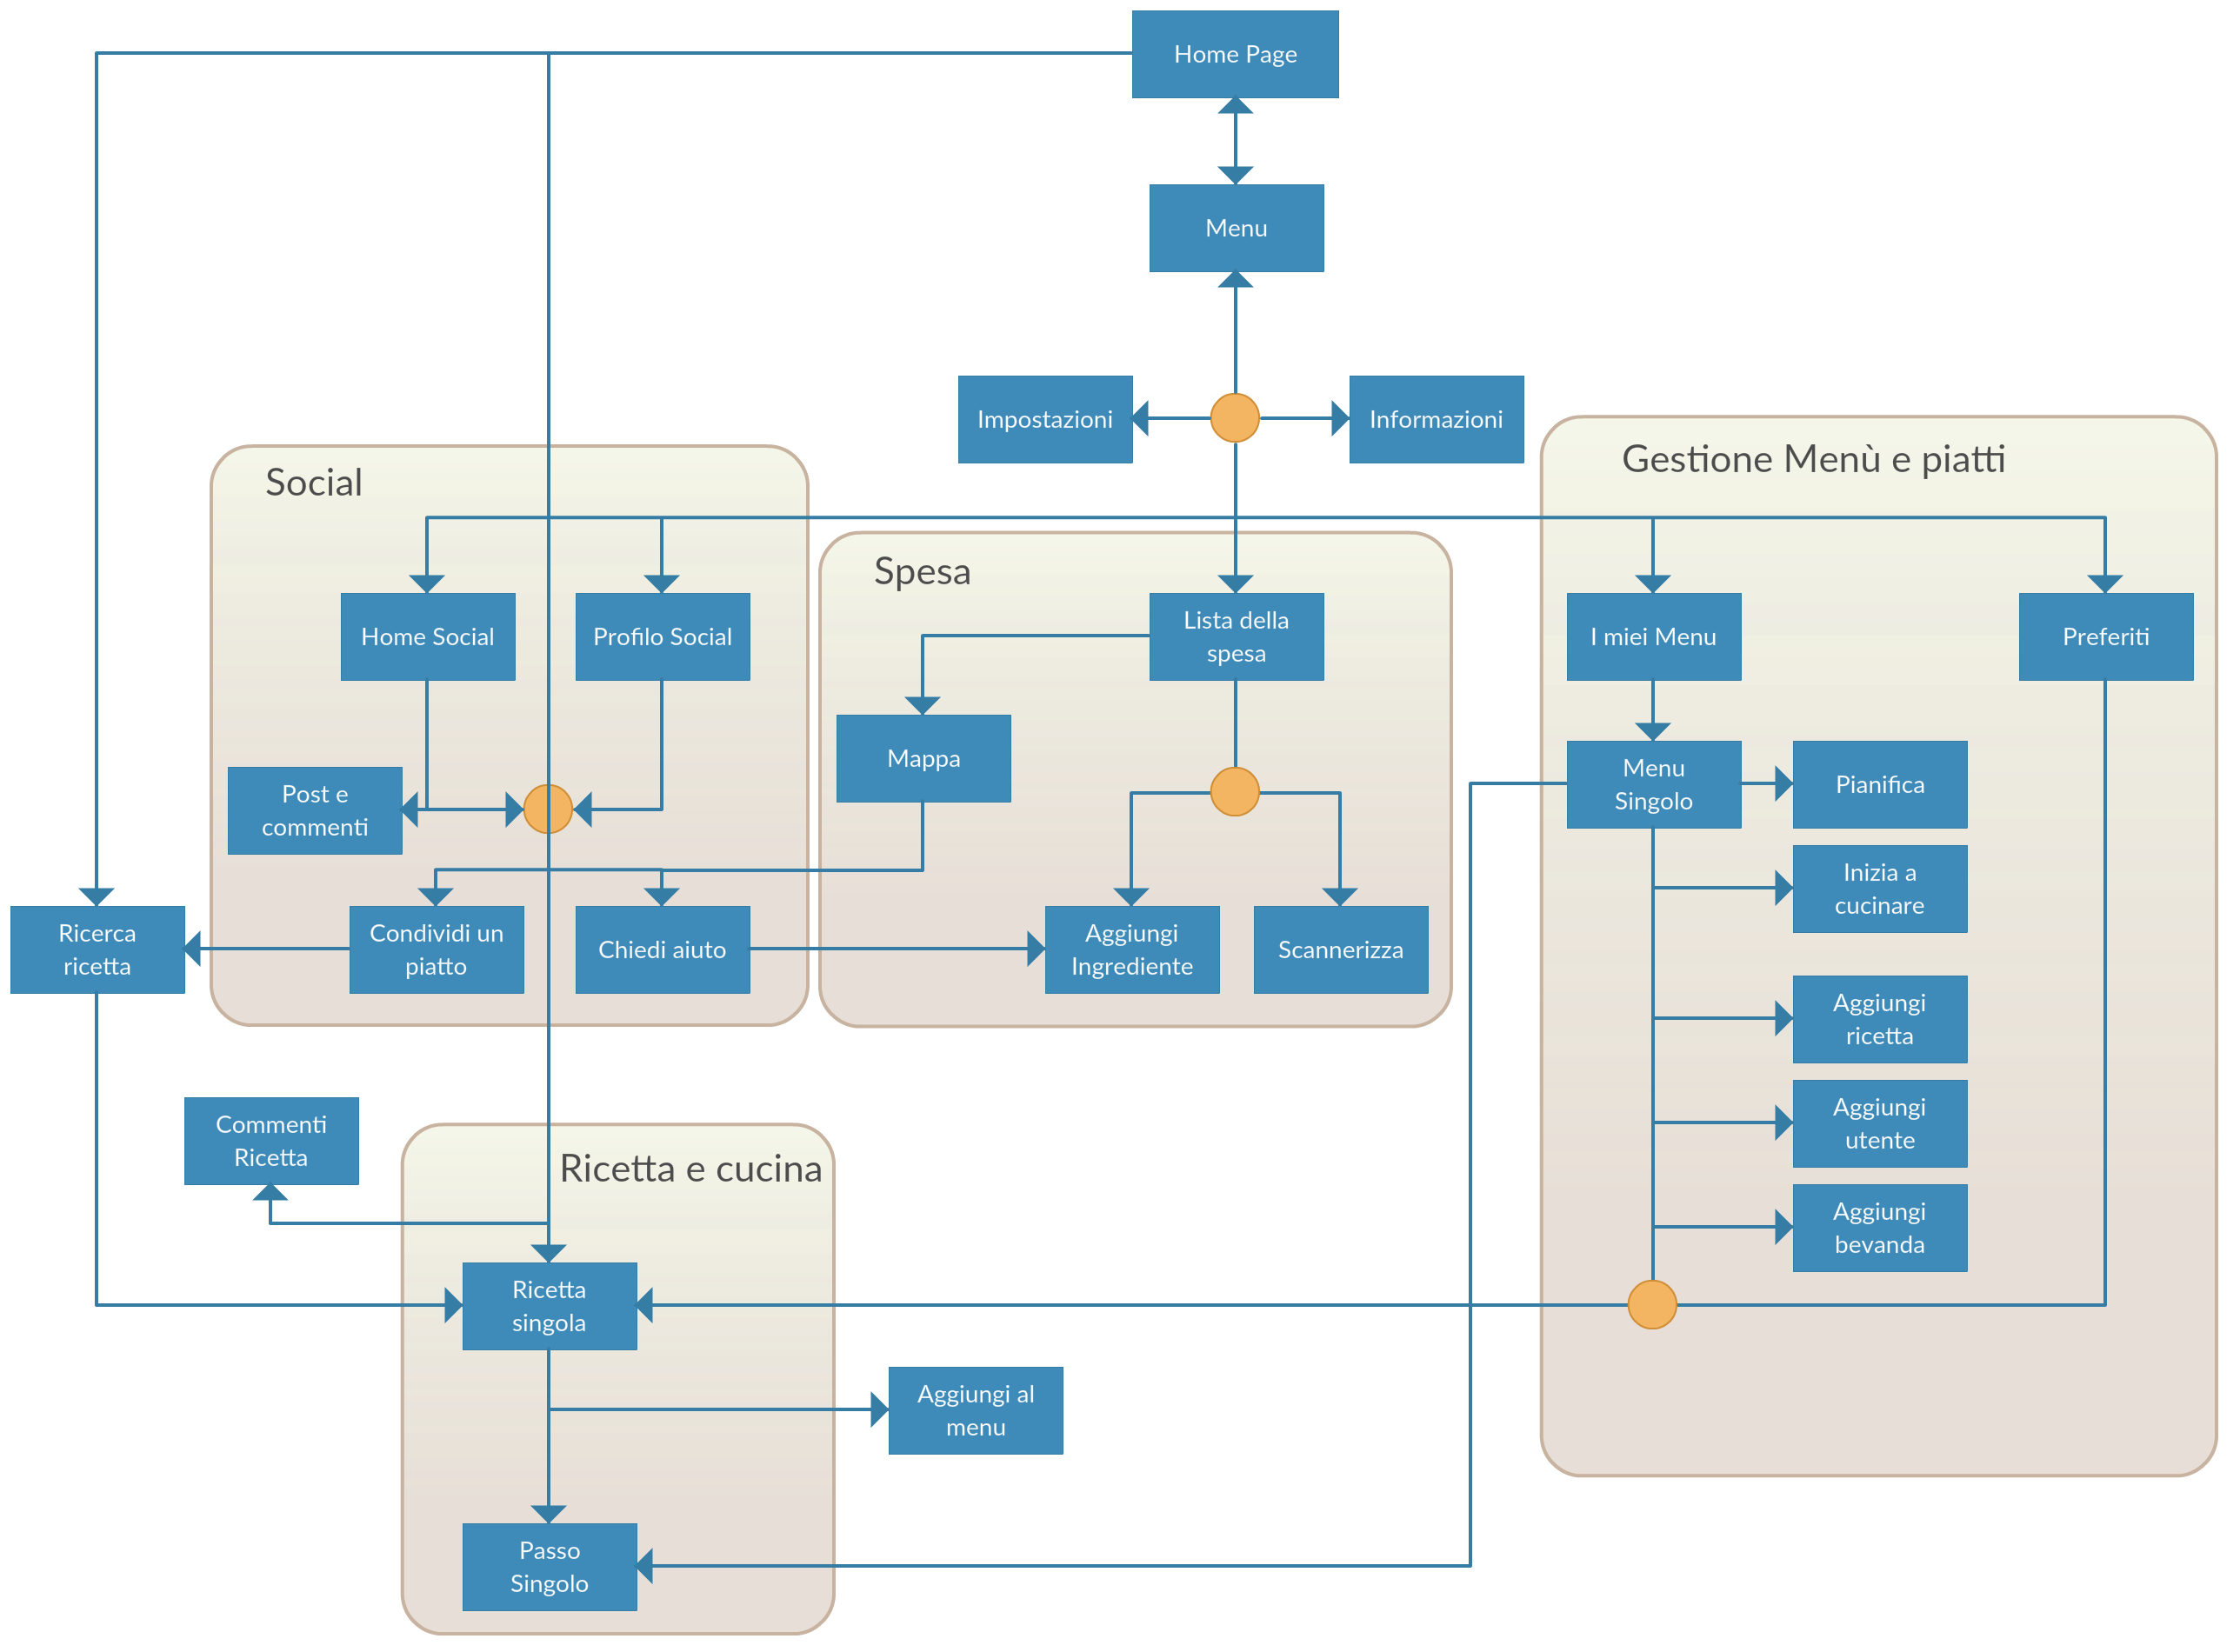
\includegraphics[width=\textwidth]{img/ipc_blueprint}
	\label{fig:blueprint}
\end{figure}
Esistono anche interazioni non specificate nel bluprint poiché troppo specifiche
alla sequenza delle interazioni, esse sono:
\begin{itemize}
	\item Premendo il tasto ``indietro" la schermata passa, ovviamente, alla
	schermata precedente, e così a ritroso fino alla schermata Home.
	Premendo nuovamente il tasto indietro (ove disponibile) in questa
	schermata verrà chiusa l'applicazione.
	\item La notifica contestuale interna all'applicazione non viene
	indicata all'interno del blueprint.
	\item La ricerca è considerata come contestuale, nell'area social
	verranno cercati gli utenti, mentre nelle altre aree verranno cercati i
	singoli piatti (rimandando alla schermata di ricerca avanzata)
	o gli ingredienti.
\end{itemize}
